%%% Preamble
\documentclass[paper=letter, fontsize=11pt]{scrartcl}
\usepackage[T1]{fontenc}
\usepackage{fourier}
\usepackage[space]{grffile}
\usepackage[english]{babel}
\usepackage[protrusion=true,expansion=true]{microtype}	
\usepackage{amsmath,amsfonts,amsthm}
\usepackage[pdftex]{graphicx}
\usepackage{url}
\usepackage{graphicx}
\usepackage{listings}
\usepackage{caption}
\usepackage{pdflscape}
\usepackage{amsmath}
\usepackage{subcaption}
\usepackage{float}
\usepackage{comment}
\usepackage{amsmath}
\setcounter{tocdepth}{3}
\usepackage{color}
\definecolor{identifierColor}{rgb}{0.65,0.16,0.16}
\lstset{identifierstyle=\color{identifierColor}}

%%% Custom sectioning (sectsty package)
\usepackage{sectsty}
\allsectionsfont{\centering \normalfont\scshape}

\usepackage[top=1in, bottom=1in, left=1in, right=1in]{geometry}

%%% Custom headers/footers (fancyhdr package)
\usepackage{fancyhdr}
\pagestyle{fancyplain}
\fancyhead{}
\fancyfoot[C]{}
\fancyfoot[R]{\thepage}							% Pagenumbering


\renewcommand{\headrulewidth}{0pt}				% Remove header underlines
\renewcommand{\footrulewidth}{0pt}				% Remove footer underlines
\setlength{\headheight}{13.6pt}


%%% Equation and float numbering
\numberwithin{equation}{section}		% Equationnumbering: section.eq#
\numberwithin{figure}{section}			% Figurenumbering: section.fig#
\numberwithin{table}{section}			% Tablenumbering: section.tab#


%%% Maketitle metadata
\newcommand{\horrule}[1]{\rule{\linewidth}{#1}}
\title{
		\vspace{-1in} 	
		\usefont{OT1}{bch}{b}{n}
		\normalfont \normalsize \textsc{ME/EE Design Capstone 450} \\ [25pt]
		\horrule{0.5pt} \\[0.4cm]
		\huge Final Report\\
		\horrule{2pt} \\[0.5cm]
}
\author{
        \normalfont 							
        \normalsize
        Edited by: \\
        Sam Li \\ limutian@yahoo.com \\[2pt]
        Sasha Sheng \\ sasha@sashasheng.com\\[2pt]
        Christina Yan \\ yyoucai@umich.edu\\[2pt]
        Siyuan Zhang\\ kevin.zhangsiyuan@gmail.com\\[2pt]
        Wang Zi \\ waziprince@163.com\\ [5pt]
        Sponsored: \\ Dr. Shane Johnson,  shane.johnson@sjtu.edu.cn\\ \vspace{0.5cm}
}

%%% Begin document
\begin{document}
\maketitle
\begin{figure}[H]
    \centering
    
\includegraphics[scale=0.7]{LOGO.png}
\end{figure}
\pagebreak
\tableofcontents
\pagebreak
	
\section{Revised Abstract}	
In this paper, a new design for analyzing blood perfusion is introduced. Unlike current medical solution such as using Laser Doppler Imaging or Noninvasive near-infrared spectroscopy, infrared camera is used to detect the temperature difference of human surface skin which is caused by an internal excitation, the heartbeats. Two set-up for simulating human skin would be built for experiments, one with latex tubing and another with stainless steel, which would be introduced in detail in the paper. These set-ups generate same effects as human body does and the data processed is valuable to be studied to approach the final result.

\section{Introduction}
This section briefly introduces the problem we want to solve, an introduction to our project, the aims and goals we want to achieve, and also analysis about our competitors.
\subsection{Problem Description}
In this paper, a new design for analyzing blood perfusion is introduced. Unlike current medical solution such as using Laser Doppler Imaging or Noninvasive near-infrared spectroscopy, infrared camera is used to detect the temperature difference of human surface skin which is caused by an internal excitation, the heartbeats. Two set-up for simulating human skin would be built for experiments, one with latex tubing and another with stainless steel, which would be introduced in detail in the paper. These set-ups generate same effects as human body does and the data processed is valuable to be studied to approach the final result.
\subsection{Project introduction}
We aim to develop a system based on infra-red camera to evaluate human blood perfusion, which will hopefully be a much cheaper solution to some medical problems including evaluating burn depth, tumor and so on. The system takes infra-red pictures at a fixed frame rate for a specific time period, and we analyze the pictures in order to get the temperature fluctuation($\delta T$) at each point(pixel) in the picture. Our goal is to get one final image that shows clearly the $\delta T$ for each pixel.
\subsection{Aims and Goals}
We are developing a system that is inexpensive, easy to use and provides accurate results in inspecting blood perfusion for medical purposes. Our system takes infrared pictures, which after being analyzed provides information about blood perfusion.
\subsection{Competitors}
Previous research works on using active-dynamic infrared thermal imaging (ADT) to evaluate perfusion and burn depth have shown that infra-red pictures can provide accurate results in discriminating burn depths \cite{Renkielska}\cite{Ruminski}. The ADT method applies an external excitation (heat/light) to the wound area, and then uses infrared camera to look at thermal transients at the surface of the wound, which can be used to determine the burn wound depth \cite{Renkielska}\cite{Ruminski}. Our system is different from these infra-red methods mainly in that we do not use an external excitation source. Using an infra-red camera with higher accuracy, we will be able to monitor the spontaneous fluctuation of human body temperature, which goes up when the heart pumps blood to the body, and drops between heart beats. We trigger the infra-red camera to take a series of pictures when body temperature rises, thus using human heart beat as the internal excitation source. Based on the same principle as ADT, we expect our method to also provide accurate evaluations of blood perfusion. Our final set-up is simpler than ADT methods because we do not need external excitation source. This also means less pain for the patient because we do not stimulate the already wounded area. We also expect lower noise-signal ratio for our method because we do not have to filter out the meaningless reflection signal caused by external excitation, which is noise for the system. In the ADT method devoted work has to be done to deal with such noise \cite{Ruminski}. Our result should be more accurate because we operate in a smaller temperature range, which is determined by the spontaneous fluctuation of human body temperature.
\section{Experiment Set-up}
Before testing on human body, prototypes are made to try out the basic idea for the reason that it is easier to manipulate the parameters in a relatively ideal condition.
There are basically two plans for simulating the human body to be tested. Referring to the paper and professional�s advices, both the prototypes are of a sandwich-like structure. It contains a heat sink as the base, the silicon layer as the top membrane and vessel in between. The only difference between the two plans is the method of mimicking the blood and vessel.
\subsection{First Plan}
The first one is liquid-based. The polythene tube and heated saline solution are for mimicking the vessel and blood. The system is consisted of three parts: the flesh and vessel, the pump and water bath bucket.
\subsubsection{Flesh and Vessel}
This part is constructed as a sandwich structure. The base is made of a 25mm gelatin layer. It is proper heat sink and absorber just as the human flesh. A 3mm-inner diameter polythene tube is bended and arranged in between the gelatin base and top silicon layers.  The two components need to be mixed together in a box. Referring to the thickness of the skin, we made it 2mm thick. According to the previous experience, anything thicker than 2mm will prevent heat dissipating of the blood. The industrial blower is applied to provide hot air in order to accelerate its solidification. This step approximately takes 10-15 minutes regarding to its thickness and room temperature of 26-Celsius degrees. After making this silicon layers, we meticulously configured the tube in Z shape and enclose the layers altogether. As the material is sticky and soft even after its complete solidification, it is necessary to keep it insulated in a clean, cool and dry spot. After 1~2 hours� standing, this piece of flesh is integrated. 

\begin{figure}[H]
    \centering
    \begin{minipage}[t]{0.44\textwidth}
        \centering
        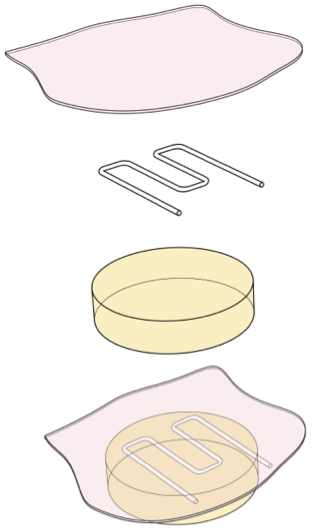
\includegraphics[scale=0.8]{1}
        \caption{2D schematic of Skin Simulation}
    \end{minipage}
    \begin{minipage}[t]{0.44\textwidth}
        \centering
        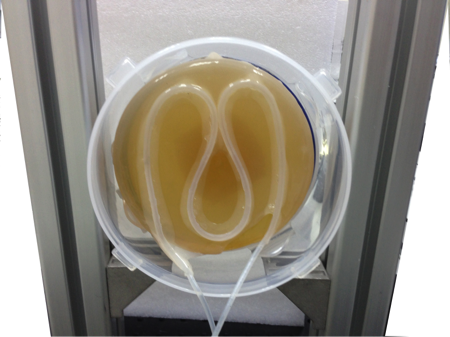
\includegraphics[scale=0.8]{2}
        \caption{Physical Setup of Skin Simulation}
    \end{minipage}
\end{figure}

\subsubsection{Peristaltic Pump}
The pump responses for absorbing the saline solution from the water bath tank into the flesh module. Here are some reasons why we chose this kind of pump.
As the blood perfusion is generated pulse by pulse, the peristaltic has the feature of providing impulse that we are seeking for, which needs to be eliminated in many circumstances somehow. Here is a diagram showing its working principle.\cite{peristaltic_pump}
\subsubsection{Water bath bucket}
It needs to be adjustable and as sensitive as +/- 0.1$^\circ$ C
The following diagram shows the connection.

\begin{figure}[H]
    \centering
    \begin{minipage}[t]{0.5\textwidth}
        \centering
        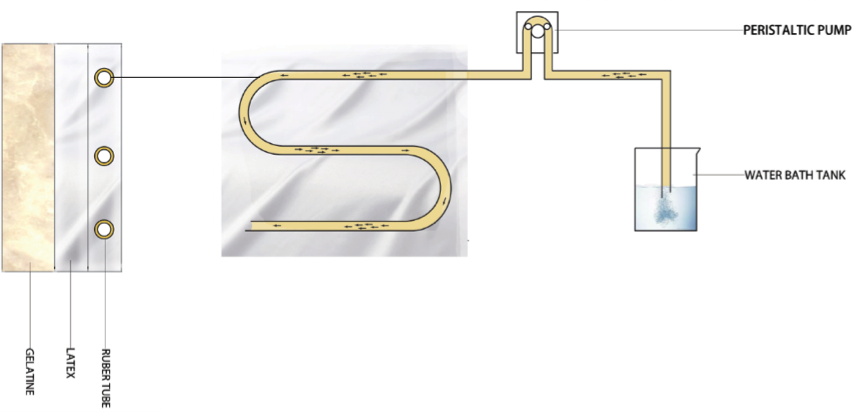
\includegraphics[scale=0.8]{3}
        \caption{2D schematic}
    \end{minipage}
    \begin{minipage}[t]{0.5\textwidth}
        \centering
        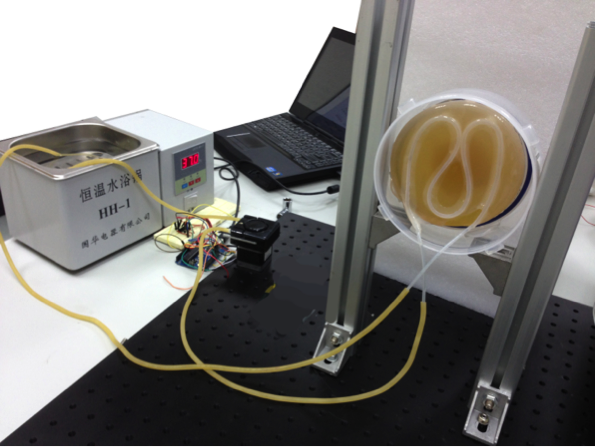
\includegraphics[scale=0.8]{4}
        \caption{Physical Setup}
    \end{minipage}
\end{figure}

\subsection{Second Plan}
This second plan is voltage-based.
Compared with the first design, the tube (2mm outer diameter, 1mm inner diameter) and heated solution is altered by the stainless steel stripe with a waved signal applied.  Stainless steel is a poor conductor material so that it can work as a resistant to accumulate heat. It is connected to a function generator where a square wave is produced onto the stripe in order to simulate the periodical blood perfusion. The temperature of stripe should also fluctuate periodically.
The setup is shown in the following diagram.
\begin{figure}[H]
    \centering
    \begin{minipage}[t]{0.33\textwidth}
        \centering
        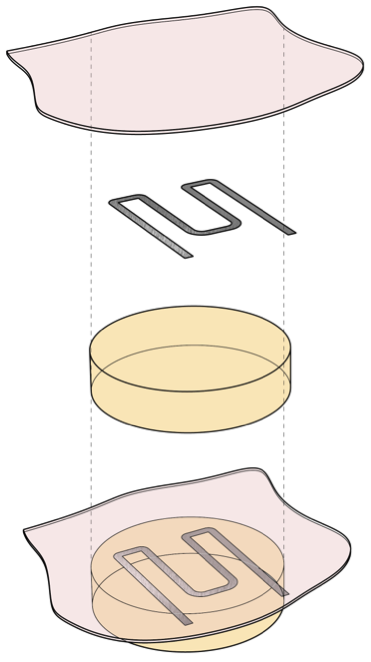
\includegraphics[scale=0.5]{5}
        \caption{3D Schematic of Skin}
    \end{minipage}
    \begin{minipage}[t]{0.33\textwidth}
        \centering
        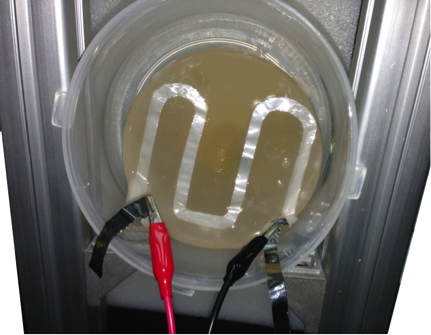
\includegraphics[scale=0.5]{6}
        \caption{Physical Setup of Skin}
    \end{minipage}
 \end{figure}

     \begin{figure}[H]
             \centering
        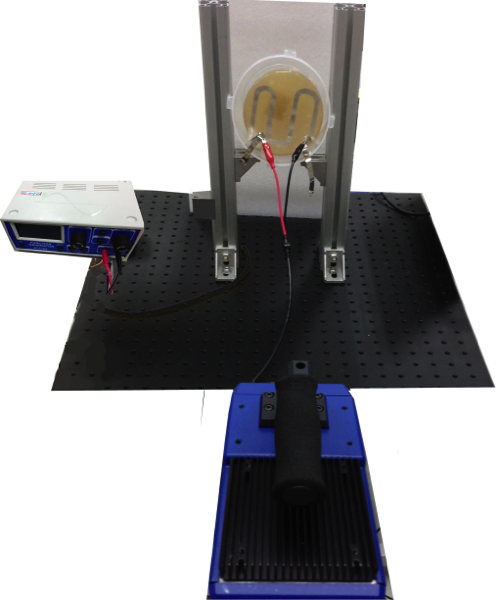
\includegraphics[scale=0.8]{7}
        \caption{Total Setup}
\end{figure}

\section{Triggering}
This section introduce the method to trigger FLIR A325 and SC7700. Both of these infrared camera have recording trigger function which can be triggered by pulse of voltage to save data.
\subsection{Hardware connection}
\subsubsection{Camera to MyDAQ}
\begin{figure}[H]
    \centering
    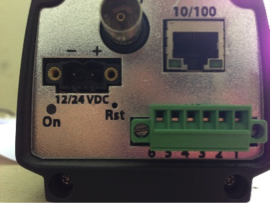
\includegraphics[scale=1]{8}
    \caption{MyDAQ Connections}
\end{figure}
For A325, there are six I/O ports. The input port 1 (IN1) is used to start the trigger for recording and input port 2 (IN2) is used to stop the trigger for recording. And port 6 is the GND. Other ports won't be used for trigger function. As manual introduces, the state (high or low voltage) on an input pin is used to start an event in the camera, to be specifically, 0 - 1.5V = low and 3 - 25 V = high for two input ports. So we can use pulse or square wave which has amplitude of 0-5v as trigger signal. If we use MyDAQ as signal generator, just connect IN1 to the output port on MyDAQ you set, e.g. DO(digital output)0, and connect port 6 to GND.
\begin{figure}[H]
    \centering
    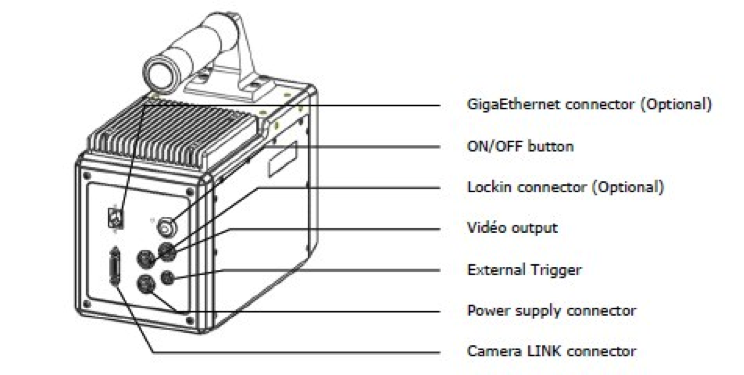
\includegraphics[scale=0.7]{9}
    \caption{Camera Connections}
\end{figure}
For SC7700, the external trigger port has connector that can be transferred to BNC port. To connect BNC male port to our signal, the central pin goes to positive output of MyDAQ, and the other pin goes to the GND. And this port can be triggered by voltage over 3.3V. 
\begin{figure}[H]
    \centering
    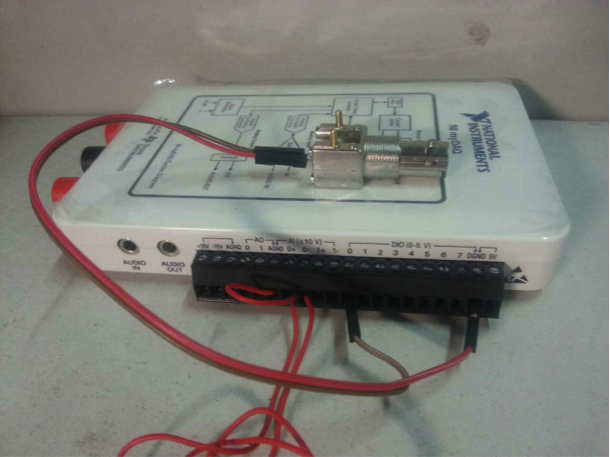
\includegraphics[scale=0.7]{10}
    \caption{Connection Head with Camera}
\end{figure}
\subsubsection{MyDAQ to ECG}
We use MyDAQ to acquire signal from ECG. We use AI (analog input) ports on MyDAQ, 0+ connect to the positive output of ECG, and 0- connect to the negative output of ECG, then connect 0- to the GND on MyDAQ.
\subsection{Software}
\subsubsection{LabVIEW}
Here we use LabVIEW both to acquire and generate signal. We acquire heart beats signal from ECG, and generate a square wave to trigger the infrared camera. In general, we use a same time line to record data of ECG signal and trigger signal, write them into the same file, and then analyze the data. The specific design diagram will be included in Appendix.
\subsubsection{FLIR Research IR Max}
FLIR ResearchIR is aimed at R\&D-Science users of thermal imaging cameras with a cooled or uncooled detector. It supports both A325 and SC7700. To connect A325 to your computer, you need FLIR IP Config to detect its IP address, and set IP address of your IPV4 to the same address of camera, only change the last digit (e.g. if camera IP is 192.168.1.250, you can set your IP as 192.168.1.245). For SC7700, you can just set as obtain IP address automatically. Then software can detect and connect the camera. Then we go to triggering method, set start trigger as external trigger, and stop trigger by external trigger of other method, like duration or number of frame. If we choose automatically rearm the trigger, we can trigger it every time the square wave goes to high voltage, otherwise it can only be triggered once. The highest frame rate of A325 is 60Hz, and 117Hz for SC7700. However, when we try to trigger the camera with the signal that has such high frequency, we found that the camera can be triggered only about 2Hz. It can take 60 frame per triggered, so we can still get a frame rate of 60Hz theoretically. In real experiment, we adjust the frequency of trigger signal and the number of frame per triggered in order to get the highest frame rate.

\section{Experiments and Data Analysis}
Experiments were done with real human body, the stainless steel system and the latex tubing system respectively. In the following experiments FLIR SC7700 camera were used. The data generated by Infra-red camera is PTW file that consists of multiple frames. Each frame is represented by a 512*640 array of photon flux values.
\subsection{Experiment 1: Human Hand}
We took pictures of human hand at 25 frames per second. We looked at data for 16 seconds (400 frames). In each frame, we took pixels with relatively high values, and calculated mean value of those pixels. Plotting this mean value with respect to the 400 frames showed that the temperature of most active parts (blood veins) indeed fluctuated at a rate of approximately 1 Hz, which corresponds to the frequency of human heart beat.
\begin{figure}[H]
	    \centering
	\begin{subfigure}[t]{0.33\textwidth}
        \centering
        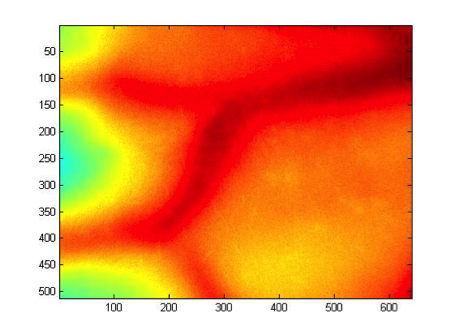
\includegraphics[scale=0.7]{11}
    \end{subfigure}
    \begin{subfigure}[t]{0.33\textwidth}
        \centering
        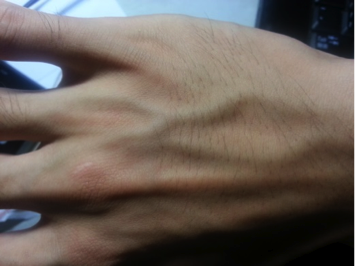
\includegraphics[scale=0.7]{12}
    \end{subfigure}
	\caption{Human hand in the experiment (and Infra-red image)}
\end{figure}

\begin{figure}[H]
    \centering
    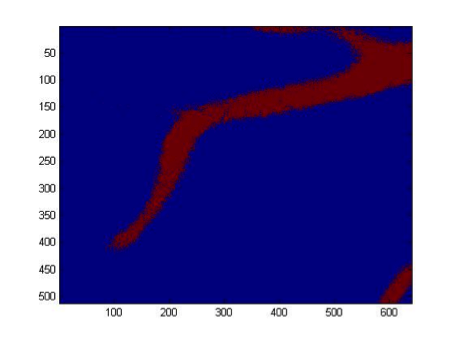
\includegraphics[scale=1]{13}
    \caption{Pixels with Relatively High Values (indicated in red)}
\end{figure}

\begin{figure}[H]
    \centering
    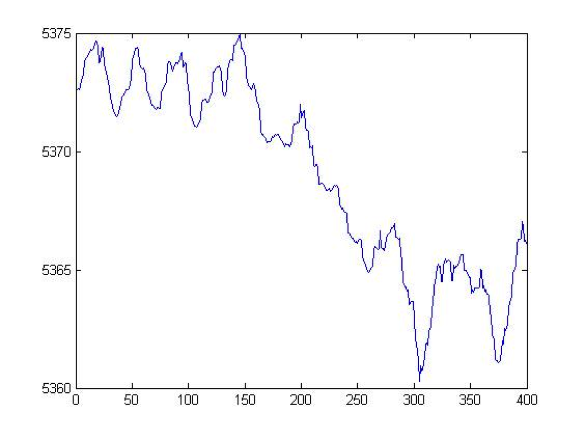
\includegraphics[scale=1]{14}
    \caption{Plot of Mean Values in Each Frame}
\end{figure}
We also looked at the amplitude of the temperature fluctuation($\delta T$) for each pixel. For each pixel across the 400 frames, we applied a simple algorithm to find the peaks and valleys of the data. We used the difference between the mean values of the peaks and valleys as $\delta T$ for that pixel, and processed each pixel this way. Finally we got one 512*640 array, with a $\delta T$ value in each pixel. Fig 5.4 is an image that represents the array (brighter color represents higher $\delta T$ value).

\begin{figure}[H]
    \centering
    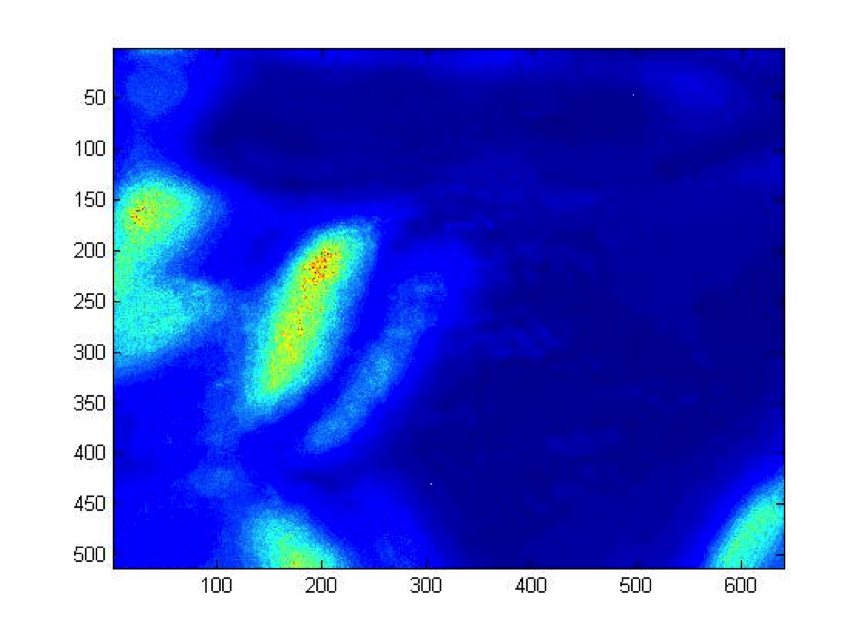
\includegraphics[scale=1]{15}
    \caption{Average $\delta T$ image}
\end{figure}

We expected high  $\delta T$ values in vein regions, because blood perfusion causes larger temperature fluctuation in these regions. From Figure 5.4 we see that the high  $\delta T$ regions are vein regions, but not all veins are highlighted by high  $\delta T$ values. This is because when we look at each pixel across the 400 frames, the data becomes noisy and reflects temperature change that is not at about 1 Hz. Therefore the peaks and valleys algorithm doesn't give optimal $\delta T$ values. If we had more time, we could improve the algorithm to only look at frequency of about 1 Hz, which would produce more accurate  $\delta T$ values.

\subsection{Experiment 2: Stainless Steel System}
In this experiment we applied square wave voltage to two sides of stainless steel strip to simulate the heat generated by blood perfusion in human body. Pictures are taken at 50 frames per second. We looked at data for 8 seconds (400 frames).
\begin{figure}[H]
    \centering
    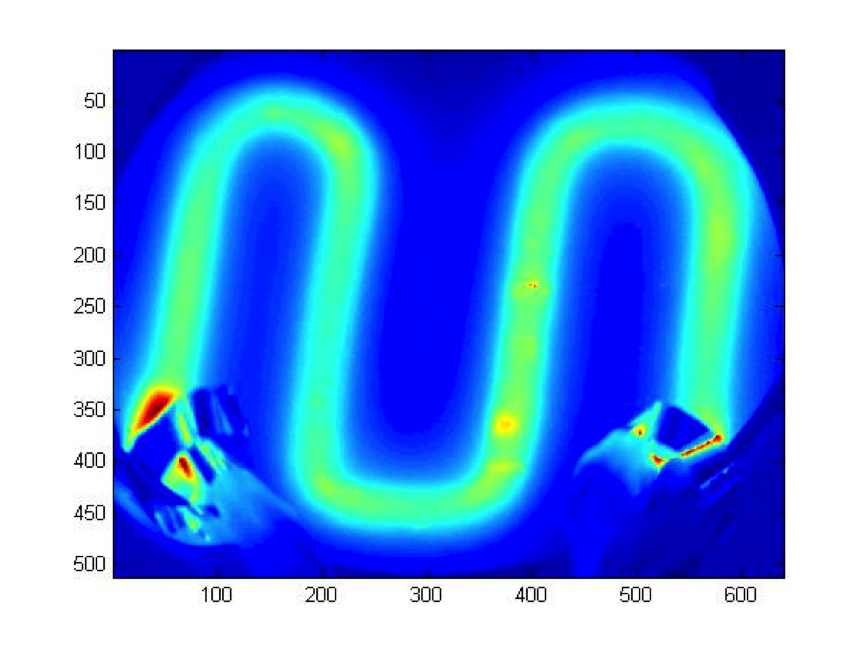
\includegraphics[scale=0.7]{16}
    \caption{Infra-red image of stainless steel system}
\end{figure}
Looking at only pixels with relatively high photon flux values, and taking their mean values for each frame and then plotting this mean with respect to 400 frames gives the following figure.
\begin{figure}[H]
    \centering
    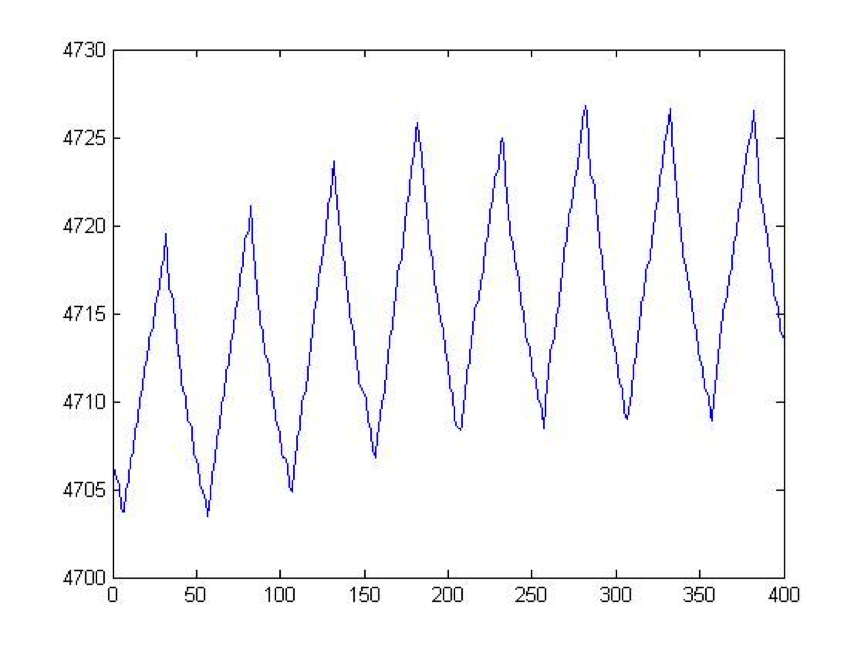
\includegraphics[scale=0.7]{17}
    \caption{Plot of Mean Values in Each Frame}
\end{figure}

\subsection{Experiment 3: latex tubing system}
This experiment looked at the latex tubing system. Saline solution was pumped inside the latex tubing by a peristaltic pump rotating at 96 rpm.  A water bath bucket was used to keep the solution at 36.8 degrees Celsius, which is human body temperature. Pictures were taken at 100 frames per second, and we looked at data for 22.35 seconds (2235 frames).
\begin{figure}[H]
    \centering
    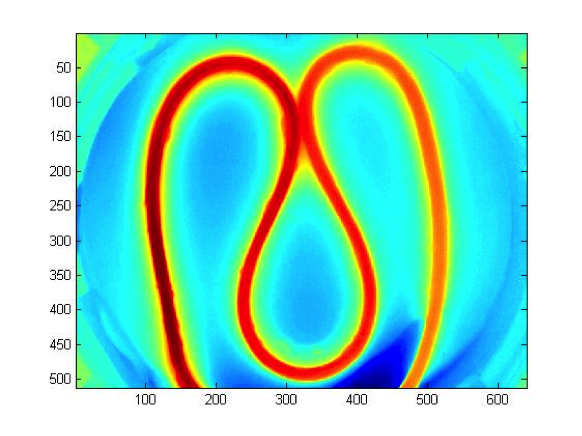
\includegraphics[scale=0.7]{18}
    \caption{Infra-red image of latex tubing system}
\end{figure}
Applying the algorithm of taking the mean value of only relatively high values in each pixel and plotting the mean values across the 800 frames, we got the following figure.
\begin{figure}[H]
    \centering
    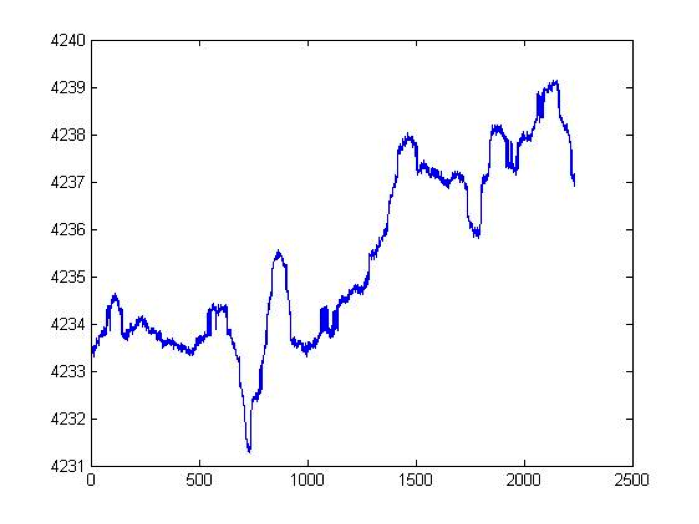
\includegraphics[scale=0.7]{19}
    \caption{plot of mean values in each frame}
\end{figure}
We can see that there was temperature fluctuation at undesired frequencies. This was because it took very long time for the system to reach equilibrium, and overall temperature in the system was still rising when we took the pictures. Therefore the result is not good.

\section{Discussion}
From the experiments, we see that the FLIR SC7700 camera is sensitive enough to capture the temperature fluctuation caused by human blood perfusion, which is very exciting. Data analysis shows that regions with stronger blood perfusion(veins) exhibit larger temperature fluctuation ($\delta T$). However, the algorithm needs to be improved in order to get more accurate $\delta T$ values for each pixel.

Taking ECG signal into account in the data analysis would also help in getting a better $\delta T$ image. This is because we are only interested in temperature changes due to blood perfusion, which is caused by heart beats. ECG signal is more information in the system to help filtering out undesired frequencies and getting the $\delta T$ that is of interest.

\section{Conclusions}
In order to analyze the temperature change in the human body with respond to heart beats, we built two systems (as discussed in Experimental Setup). However, from the analysis in the previous section. The only result we can get from the two simulation experiments are that the camera is sensitive enough to produce such cyclic images and data with minor temperature change. Here are some of the reasons why the two experiments aren't as successful as directly analyzing human hand and a few points that need to noted in future experiments:

\begin{enumerate}
\item Pay close attention to data instead of the graph. Usually data points give a more accurate results.
\item Gelatin is easy to get mold. Put it in the refrigerator if it isn't being used.
\item Silicon skin should be as close as possible to 2mm,  human skin thickness.
\item The diameter of the tubes that serves as vessels need to be as small as possible so that a pressure change could be induced.
\item The ECG we built was not always stable. It would be better to apply better filter or use other ways to make it more stable. Buying a working ECG is also a good choice.
\item The camera can take multiple frames after being triggered once, so there is no need to generate triggering signal with very high frequency using labview, as it would cause problems (labview while loops take certain time to execute, and there will be problems as the signal frequency gets near it).
\end{enumerate}

\pagebreak


\bibliographystyle{plain}
\bibliography{Final}
\pagebreak
\begin{landscape}
\section{Appendix - EKG}
EKG, abbreviation for Electrocardiography, is a transthoracic interpretation of the electrical activity of the heart over a period of time, which is detected by electrodes attached to the surface of the skin and recorded by a device external to the body. Usually the output the EKG is the electrocardiogram, which can be used to measure the rate and regularity of heartbeats. In our project, EKG system is used to detect signal of heartbeats for the testers. Then the electrocardiogram it outputs would be transmitted into the MyDAQ, which would record the voltage and its amplitude. The following is the diagram of EKG to build:
\begin{figure}[H]
    \centering
    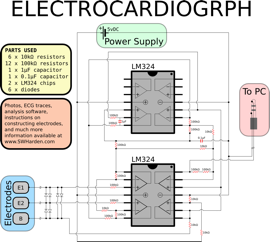
\includegraphics[scale=1]{EKG}
    \caption{EKG Schematic}
\end{figure}

\begin{figure}[H]
	\centering
	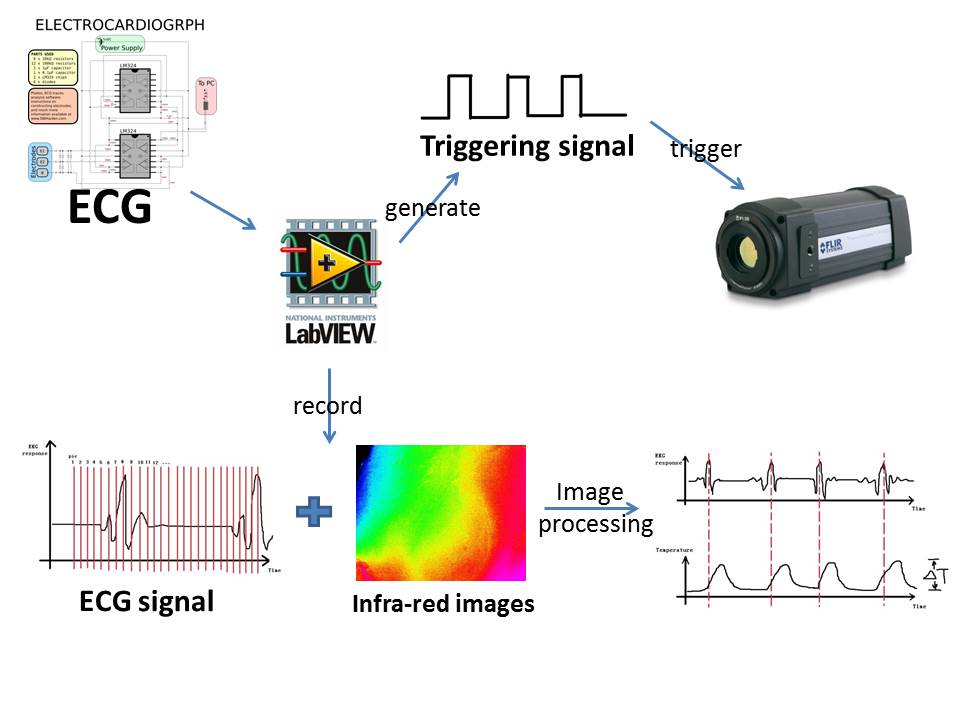
\includegraphics[scale=0.7]{Sys'}
	\caption{System Flowgram}
\end{figure}
\end{landscape}
\end{document}
